\chapter{Выбор параметров нелинейных моделей с помощью квадратичного отбора признаков}
\label{ch:newton_qpfs}

Функция ошибки для моделей с большим числом параметров имеет сложный ландшафт с многими локальными минимумами.
В этом случае алгоритм оптимизации приводит к разным решениям в зависимости от инициализации исходных параметров.

Алгоритм оптимизации представляет собой итерационный процесс.
На каждом шаге для получения следующего приближения параметров модели обновляются текущие параметры.
Разработано множество алгоритмов оптимизации первого порядка, использующих вектор первых производных функции ошибки.
Наиболее известными алгоритмами являются градиентный спуск, 
метод момента Нестерова~\cite{nesterov1983momentum}, AdaGrad~\cite{duchi2011adagrad}, Adam~\cite{kingma2014adam}.
Данные алгоритмы используются для оптимизации глубоких нейронных сетей~\cite{goodfellow2016deeplearningbook}.
Метод Ньютона~--- алгоритм второго порядка, использующий матрицу вторых производных функции ошибки.
Метод Ньютона находит обновления параметров для квадратичной аппроксимации функции ошибки и сходится за адекватное число итераций.
Недостатком методов оптимизации второго порядка является огромная и плохо обусловленная матрица Гессиана.
Процесс оптимизации в этом случае расходится и является вычислительно дорогостоящим.
Авторы~\cite{avriel2003nonlinear,blaschke1997convergence} предлагают аппроксимации для матрицы Гессиана и регуляризацию для решения этой проблемы.
В статье~\cite{botev2017newtondeeplearning} метод Ньютона применяется к глубоким нейронным сетям.

В данной главе приводится анализ параметров модели, которые не находятся в оптимуме.
Приводится метод выбора активных параметров модели, основанный на алгоритме QPFS, который подробно описан в главе~\ref{ch:qpfs}.
Рассматриваются задачи нелинейной регрессии с квадратичной функцией потерь, логистической регрессии с кросс-энтропийной функцией потерь.  

%%%%%%%%%%%%%%%%%%%%%%%%%%%%%%%%%%%%%%%%%%%%%%%%
\section{Задача выбора параметров для обучения моделей}
\label{sec:ch4:newton_qpfs_param_selection}
%%%%%%%%%%%%%%%%%%%%%%%%%%%%%%%%%%%%%%%%%%%%%%%%

Функция ошибки для моделей с большим числом параметров имеет сложный ландшафт с многими локальными минимумами.
В этом случае алгоритм оптимизации приводит к разным решениям в зависимости от инициализации исходных параметров.

Алгоритм оптимизации представляет собой итерационный процесс.
На каждом шаге для получения следующего приближения параметров модели обновляются текущие параметры.
Разработано множество алгоритмов оптимизации первого порядка, использующих вектор первых производных функции ошибки.
Наиболее известными алгоритмами являются градиентный спуск, 
метод момента Нестерова~\cite{nesterov1983momentum}, AdaGrad~\cite{duchi2011adagrad}, Adam~\cite{kingma2014adam}.
Данные алгоритмы используются для оптимизации глубоких нейронных сетей~\cite{goodfellow2016deeplearningbook}.
Метод Ньютона~--алгоритм второго порядка, использующий матрицу вторых производных функции ошибки.
Метод Ньютона находит обновления параметров для квадратичной аппроксимации функции ошибки и сходится за адекватное число итераций.
Недостатком методов оптимизации второго порядка является огромная и плохо обусловленная матрица Гессиана.
Процесс оптимизации в этом случае расходится и является вычислительно дорогостоящим.
Авторы~\cite{avriel2003nonlinear,blaschke1997convergence} предлагают аппроксимации для матрицы Гессиана и регуляризацию для решения этой проблемы.
В статье~\cite{botev2017newtondeeplearning} метод Ньютона применяется к глубоким нейронным сетям.

Модель $f( \bx, \btheta)$ с параметрами $\btheta \in \mathbb{R}^p$ предсказывает целевую переменную~$y \in \bbY$ по объекту~$\bx \in \bbR^{n}$. Пространство~$\bbY$ представляет собой бинарные метки классов~$\{0, 1\}$ для задачи двухклассовой классификации и~$\bbR$ для задачи регрессии.
Даны матрица плана~$\bX = [\bx_1, \dots, \bx_m]^{\T} \in \bbR^{m \times n}$ и целевой вектор~$\by = [y_1, \dots, y_m]^{\T} \in \bbY^{m}$. 
Цель состоит в нахождении оптимальных параметров~$\btheta^*$.
Параметры~$\btheta$ вычисляются минимизацией функции ошибки:
\begin{equation}
\btheta^* = \argmin_{\btheta \in \bbR^p} \cL(\btheta, \bX, \by).
\label{ch3:eq:error_function}
\end{equation}
В качестве функции ошибки~$\cL (\btheta, \bX, \by)$ рассматриваются квадратичная ошибка для задачи регрессии:
\begin{equation}
\cL(\btheta, \bX, \by) = \frac 12 \| \by - \mathbf{f}(\bX, \btheta) \|_2^2 = \frac 12 \sum_{i=1}^m \bigl( y_i - f(\bx_i,  \btheta)\bigr)^2,
\label{ch3:eq:squared_error}
\end{equation}
и функция кросс-энтропии для задачи бинарной классификации: 
\begin{equation}
\cL(\btheta, \bX, \by) = \sum_{i=1}^m \bigl[y_i \log f (\bx_i , \btheta) + (1-y_i) \log \bigl(1 - f (\bx_i , \btheta)\bigr)\bigr].
\label{ch3:eq:log_loss}
\end{equation}

Задача~\eqref{ch3:eq:error_function} решается с помощью итеративной процедуры оптимизации. 
Для получения параметров на шаге~$k$ текущие параметры $\btheta^{k-1}$ обновляются по следующему правилу:
\begin{equation}
\btheta^k = \btheta^{k - 1} + \Delta \btheta^{k - 1}.
\label{ch3:eq:update_rule}
\end{equation}
Авторы используют метод оптимизации Ньютона для выбора вектора обновлений~$\Delta \btheta$.

Метод Ньютона нестабилен и вычислительно сложен. 
В данной статье предлагается стабильный алгоритм Ньютона. 
Перед шагом градиента предлагается выбрать подмножество активных параметров модели, которые оказывают наибольшее влияние на функцию ошибки~$\cL (\btheta, \bX, \by)$.
Обновление параметров производится только для отобранного множества индексов~$\cA = \{j: a_j = 1, \ba \in \{0, 1\}^p\}$

\begin{align*}
\btheta_{\cA}^k &= \btheta_{\cA}^{k - 1} + \Delta \btheta_{\cA}^{k - 1}, \quad \btheta_{\cA} = \{\theta_j: j \in \cA \}; \\
\btheta_{\bar{\cA}}^k &= \bw_{\bar{\cA}}^{k - 1}, \quad \btheta_{\bar{\cA}} = \{\theta_j: j \notin \cA \}.
\end{align*}
Чтобы выбрать оптимальное подмножество индексов~$\cA$, из всех возможных $2^p - 1$~подмножеств, вводится функция ошибки
\begin{equation}
\ba = \argmin_{\ba' \in \{0, 1\}^p} S(\ba', \bX, \by, \btheta),
\label{ch3:eq:subset_selection}
\end{equation}
аналогичная функции ошибки~\eqref{ch2:eq:feature_selection} для задачи выбора признаков. 
Задача~\eqref{ch3:eq:subset_selection} решается на каждом шаге $k$ процесса оптимизации для текущих параметров~$\btheta^k$.

Алгоритм QPFS используется для решения задачи~\eqref{ch3:eq:subset_selection}.
QPFS выбирает подмножество параметров~$\ba$ для вектора обновлений~$ \Delta \btheta$, которые оказывают наибольшее влияние на вектор остатков и являются попарно независимыми.
Функция ошибки~\eqref{ch2:eq:qpfs_problem} соответствует функции ошибки~$S(\ba, \bX, \by, \btheta)$
\begin{equation}
\ba = \argmax_{\ba' \in \{1, 0\}^p} S(\ba', \bX, \by, \btheta) \Leftrightarrow \argmin_{\ba  \in \bbR^p_+, \, \|\ba\|_1=1} \bigl[\ba^{\T} \bQ \ba - \alpha \cdot \mathbf{b}^{\T} \ba \bigr].
\end{equation}
В работе показано, что для модели нелинейной регрессии с квадратичной функцией ошибки~\eqref{ch3:eq:squared_error} и для модели логистической регрессии с кросс-энтропией~\eqref{ch3:eq:log_loss}, каждый шаг оптимизации эквивалентен задаче линейной регрессии~\eqref{ch2:eq:linear_regression}.

%%%%%%%%%%%%%%%%%%%%%%%%%%%%%%%%%%%%%%%%%%%%%%%%
\section{Метод Ньютона решения задачи обучения параметров}
\label{sec:ch4:newton_algorithm}
%%%%%%%%%%%%%%%%%%%%%%%%%%%%%%%%%%%%%%%%%%%%%%%%

Метод Ньютона использует условие оптимизации первого порядка для задачи~\eqref{ch3:eq:error_function} и линеаризует градиент $S (\btheta)$
\[
\nabla S (\btheta + \Delta \btheta) = \nabla S(\btheta) + \bH \cdot \Delta \btheta = 0,
\]
\[
\Delta \btheta = - \bH^{-1} \nabla S(\btheta).
\]
где $\bH = \nabla^2 S(\btheta)$ является Гессианом матрицы функции ошибки $S(\btheta)$.

Итерация~\eqref{ch3:eq:update_rule} метода Ньютона имеет вид
\[
\btheta^k = \btheta^{k-1} - \bH^{-1} \nabla S(\btheta).
\]
Каждая итерация инвертирует матрицу Гессиана.
Мерой плохой обусловленности для матрицы Гессиана~$\bH$ является число обусловленности
\[
\kappa(\bH) = \frac{\lambda_{\text{max}}(\bH)}{\lambda_{\text{min}}(\bH)},
\]
где $\lambda_{\text{max}}(\bH), \lambda_{\text{min}}(\bH)$ являются максимальным и минимальным собственными значениями~$\bH$. Большое число обусловленности~$\kappa (\bH)$ приводит к нестабильности процесса оптимизации.
Предложенный алгоритм уменьшает размер матрицы Гессиана~$\bH$. В наших экспериментах это приводит к меньшему числу обусловленности~$\kappa (\bH)$.

Размер шага метода Ньютона может быть чрезмерно большим. Для управления размером шага обновлений добавим параметр $\eta$ в правило обновления~\eqref{ch3:eq:update_rule}
\[
\btheta^k = \btheta^{k - 1} + \eta \Delta \btheta^{k - 1}, \quad \eta \in [0, 1].
\]

Для выбора соответствующего размера шага~$\eta$ используется правило Армихо. Выбирается максимальное~$\eta$ так, чтобы выполнялось следующее условие
\[
S(\btheta^{k - 1} + \eta \Delta \btheta^{k - 1}) < S(\btheta^{k - 1}) + \gamma \eta \nabla S^{\T}(\btheta^{k-1})\btheta^{k - 1}, \quad \gamma \in [0, 0.5].
\]

\subsection*{Модель нелинейной регрессии}
Предположим, что модель $f (\bx , \btheta)$ близка к линейной в окрестности точки $\btheta + \Delta \btheta$
\[
\mathbf{f}(\bX , \btheta + \Delta \btheta) \approx \mathbf{f}(\bX , \btheta) + \bJ \cdot \Delta  \btheta,
\]
где $\mathbf{J} \in \bbR^{m \times p}$ является матрицы Якоби
\begin{equation}
\bJ = 
\begin{pmatrix}
\frac{\partial f(\bx_1 , \btheta)}{\partial \theta_1} & \dots & 
\frac{\partial f(\bx_1 , \btheta)}{\partial \theta_p} \\
\dots & \dots & \dots \\
\frac{\partial f(\bx_m , \btheta)}{\partial \theta_1} & \dots & 
\frac{\partial f(\bx_m , \btheta)}{\partial \theta_p}
\end{pmatrix}.
\end{equation}
В соответствии с этим предположением градиент~$\nabla S(\btheta)$ и Гессиан матрицы~$\bH$ функции ошибки~\eqref{ch3:eq:squared_error} равняются
\begin{equation}
\nabla S(\btheta) = \bJ^{\T} (\by - \mathbf{f}), \quad \bH = \bJ^{\T} \bJ.
\label{ch3:eq:nonlin_reg_deriv}
\end{equation}
Это приводит к методу Гаусса-Ньютона и правилу обновления~\eqref{ch3:eq:update_rule}
\[
\btheta^k = \btheta^{k - 1} + (\bJ^{\T} \bJ)^{-1}\bJ^{\T}(\mathbf{f} - \by).
\]
Вектор обновления~$\Delta \btheta$ является решением задачи линейной регрессии
\begin{equation}
\| \be - \bF \Delta \btheta \|_2^2 \rightarrow \min_{\Delta \btheta \in \bbR^{p}},
\label{ch3:eq:lin_reg_nonlin_reg}
\end{equation}
где $\be = \mathbf{f} - \by$ и $\bF = \bJ$.

В качестве нелинейной модели рассматривается модель двухслойной нейронной сеть. В этом случае модель~$f (\bx, \btheta)$ задается
следующим образом:
\[
f(\bx, \btheta) = \sigma(\bx^{\T} \bW_1) \bw_2.
\]
Здесь~$\bW_1 \in \bbR^{m \times h}$~-- это матрица весов, которые соединяют исходные признаки с $h$ скрытыми нейронами. Функция нелинейности $\sigma(\cdot)$ применяется поэлементно. Веса~$\bw_2 \in \bbR^{h \times 1}$ соединяют скрытые нейроны с выходом. 
Вектор параметров модели~$\btheta$ представляет собой объединение векторизованных матриц~$\bW_1$, $\bw_2$.

\subsection*{Модель логистической регрессии}

Для логистической регрессии модель имеет вид $f(\bx , \btheta) = \sigma(\bx^{\T} \btheta)$ с сигмоидной функцией активации~$\sigma(\cdot)$.
Градиент и Гессиан функции ошибки~\eqref{ch3:eq:log_loss} равны
\begin{equation}
\nabla S(\btheta) = \bX^{\T} (\mathbf{f} - \by), \quad \bH = \bX^{\T} \bR \bX,
\label{ch3:eq:log_reg_deriv}
\end{equation}
где $\bR$~-- это диагональная матрица с диагональными элементами $f(\bx_i , \btheta) \cdot (1 - f(\bx_i , \btheta))$.

Правило обновления~\eqref{ch3:eq:update_rule} в этом случае
\[
\btheta^k = \btheta^{k - 1} + (\bX^{\T} \bR \bX)^{-1} \bX^{\T} (\by - \mathbf{f}).
\]
Этот алгоритм известен как итеративный алгоритм взвешенных наименьших квадратов (IRLS). Вектор обновлений $\Delta \bw$ является решением задачи линейной регрессии
\begin{equation}
\| \be - \bF \Delta \btheta \|_2^2 \rightarrow \min_{\Delta \btheta \in \bbR^{p}},
\label{ch3:eq:lin_reg_log_reg}
\end{equation}
где $\be = \bR^{-1/2} (\by - \mathbf{f})$ и $\bF = \bR^{1/2}\bX$.

%%%%%%%%%%%%%%%%%%%%%%%%%%%%%%%%%%%%%%%%%%%%%%%%
\section{Метод Ньютона с выбором параметром с помощью квадратичного программирования}
\label{sec:ch4:newton_qpfs_algorithm}
%%%%%%%%%%%%%%%%%%%%%%%%%%%%%%%%%%%%%%%%%%%%%%%%

Предлагается реализовать алгоритм QPFS для решения задач~\eqref{ch3:eq:lin_reg_nonlin_reg} и \eqref{ch3:eq:lin_reg_log_reg}. 
QPFS матрица~$\bQ$ и вектор~$\bb$ имеют вид
\[
\bQ = \text{Sim} (\bF), \quad \bb = \text{Rel} (\bF, \be).
\]

Выборочный коэффициент корреляции равен нулю для ортогональных векторов.
Покажем, что в оптимальной точке~$\btheta^*$ вектор~$\be$ ортогонален столбцам матрицы~$\bF$. 
В этом случае вектор~$\bb = \text{Rel} (\bF, \be)$ равен нулю. Это означает, что член, учитывающий релевантность, в данном случае исключается.
Условие оптимизации первого порядка гарантирует это свойство для модели нелинейной регрессии
\[
\bF^{\T} \be = \bJ^{\T} (\mathbf{f} - \by) = - \nabla S(\btheta^*) = \boldsymbol{0},
\]
и для модели логистической регрессии
\[
\bF^{\T} \be = \bX \bR^{-1/2} \bR^{1/2} (\by - \mathbf{f}) = \bX^{\T} (\by - \mathbf{f}) = \nabla S(\btheta^*) = \boldsymbol{0}.
\]
Псевдокод предлагаемого алгоритма приведён в алгоритме~\ref{pc:QPFSNewton}.

\begin{algorithm}
	\caption{QPFS + Ньютон алгоритм}
	\label{pc:QPFSNewton}
	\begin{algorithmic}
		\REQUIRE $\varepsilon$~-- допустимое отклонение;\\
		\hspace{1.07cm}$\tau$~-- пороговое значение;\\
		\hspace{1.07cm}$\gamma$~-- параметр правила Армихо.
		\ENSURE $\btheta^*$;
		\STATE  инициализировать $\btheta^0$;
		\STATE $k := 1$;
		\REPEAT
		\STATE вычислить $\be$ и $\bF$ для~\eqref{ch3:eq:lin_reg_nonlin_reg} или~\eqref{ch3:eq:lin_reg_log_reg} ;
		\vspace{0.1cm}
		\STATE $\bQ := \text{Sim} (\bF)$, $\bb := \text{Rel}(\bF, \be)$, $\alpha = \frac{\overline{\bQ}}{\overline{\bQ} + \overline{\bb}}$;
		\vspace{0.1cm}
		\STATE $\ba := \argmin_{\ba \geq 0, \, \|\ba\|_1=1}\ba^{\T} \bQ \ba - \alpha \cdot \mathbf{b}^{\T} \ba$;
		\vspace{0.1cm}
		\STATE $\cA := \{j: a_j = 1\}$;
		\vspace{0.1cm}
		\STATE вычислить $\nabla S(\btheta^{k-1})$, $\bH$ для \eqref{ch3:eq:nonlin_reg_deriv} или \eqref{ch3:eq:log_reg_deriv};
		\vspace{0.1cm}
		\STATE $\Delta \btheta^{k-1} = - \bH^{-1} \nabla S(\btheta^{k-1})$;
		\vspace{0.1cm}
		\STATE $\eta := \text{ArmijoRule}(\btheta^{k-1}, \gamma)$;
		\vspace{0.1cm}
		\STATE $\btheta_{\cA}^k = \btheta_{\cA}^{k - 1} + \eta \Delta \btheta_{\cA}^{k - 1}$;
		\vspace{0.1cm}
		\STATE $k := k + 1$;
		\vspace{0.1cm}
		\UNTIL{$\frac{\| \btheta^k - \btheta^{k-1} \|}{\| \btheta^k \|} < \varepsilon$}
	\end{algorithmic}
\end{algorithm}

%%%%%%%%%%%%%%%%%%%%%%%%%%%%%%%%%%%%%%%%%%%%%%%%
\section{Анализ значимостей параметров нелинейных моделей}
\label{sec:ch4:newton_qpfs_exp}
%%%%%%%%%%%%%%%%%%%%%%%%%%%%%%%%%%%%%%%%%%%%%%%%

Целью вычислительного эксперимента является исследование свойств предложенного алгоритма и сравнение его с другими методами. 

Исследована зависимость параметров алгоритма QPFS для задач~\eqref{ch3:eq:lin_reg_nonlin_reg},~\eqref{ch3:eq:lin_reg_log_reg}. 
Предположим, что вектор параметров~$\btheta^0$ лежит вблизи оптимального вектора параметров~$\btheta^*$. 
Рассмотрим отрезок
\[
\btheta_{\beta} = \beta \btheta^* + (1 - \beta) \btheta^0; \, \beta \in [0, 1] .
\]

Сгенерируем синтетический набор данных с 300 объектами и 7 признаками для задачи логистической регрессии. 
Ландшафт функции ошибки~\eqref{ch3:eq:log_loss} на сетке двух случайно выбранных параметров показан на Рис.~\ref{ch3:fig:log_reg_error}.
Поверхность функции ошибки выпуклая с вытянутыми линиями уровня вдоль некоторых параметров модели.
Добавим случайный шум к оптимальным параметрам~$\btheta^*$, чтобы получить точку~$\btheta^0$. Поведение вектора~$\bb$ на отрезке между~$\btheta^0$ и~$\btheta^*$ показано на Рис.~\ref{ch3:fig:log_reg_b_wrt_beta}.
Компоненты~$\bb$ начинают резко уменьшаться, приближаясь к оптимальной точке.
\begin{figure}
	\centering
	\begin{minipage}{.47\textwidth}
		\centering
		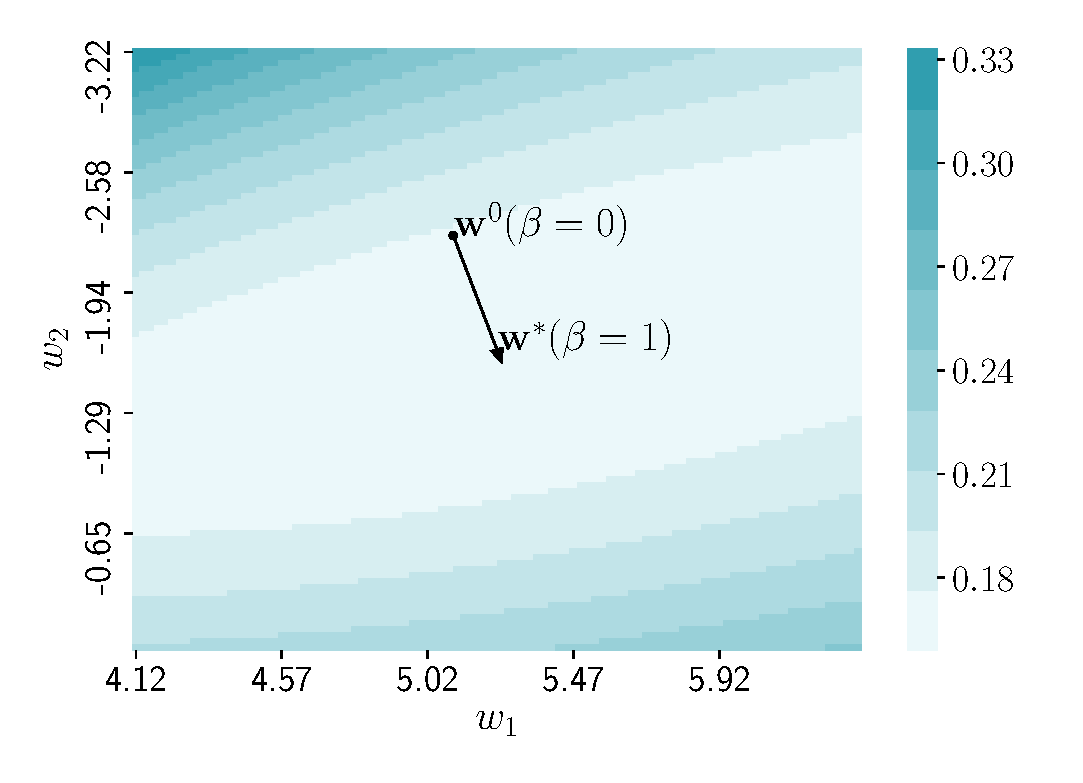
\includegraphics[width=\linewidth]{figs/ch3/log_reg_error}
		\caption{Поверхность функции ошибки для логистической регрессии}
		\label{ch3:fig:log_reg_error}
	\end{minipage}%
	\begin{minipage}{.47\textwidth}
		\centering
		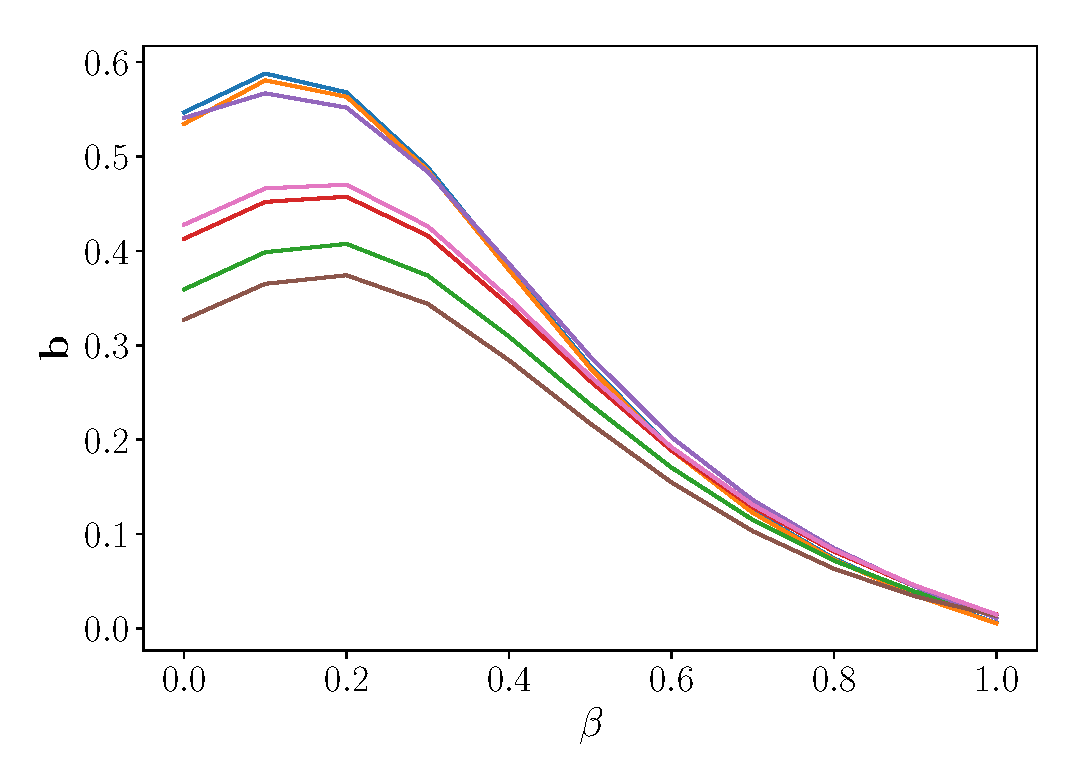
\includegraphics[width=\linewidth]{figs/ch3/log_reg_b_wrt_beta}
		\caption{Релевантность параметров для логистической регрессии}
		\label{ch3:fig:log_reg_b_wrt_beta}
	\end{minipage}
\end{figure}

Для модели нелинейной регрессии используется классический набор данных Boston Housing с 506 объектами и 13 признаками.
Для простоты нейронная сеть содержит два скрытых нейрона.
Ландшафт функции ошибок для модели нейронной сети является более сложным. 
Он не выпуклый и может содержать несколько локальных минимумов.
Двумерный ландшафт функции ошибок для этого набора данных показан на Рис.~\ref{ch3:fig:neural_error}. 
Сетка строится для двух случайных весов из матрицы~$\bW_1$.
Мы используем ту же стратегию для исследования того, как вектор~$\bb$ изменяется от~$\btheta^0$ до~$\btheta^*$. 
Результат показан на Рис.~\ref{ch3:fig:neural_b_wrt_beta}.
Компоненты вектора $\bb$ становятся близки к нулю вблизи оптимума. 
При достижении оптимального значения различные веса влияют на остатки модели~$\be$.
\begin{figure}
	\centering
	\begin{minipage}{.5\textwidth}
		\centering
		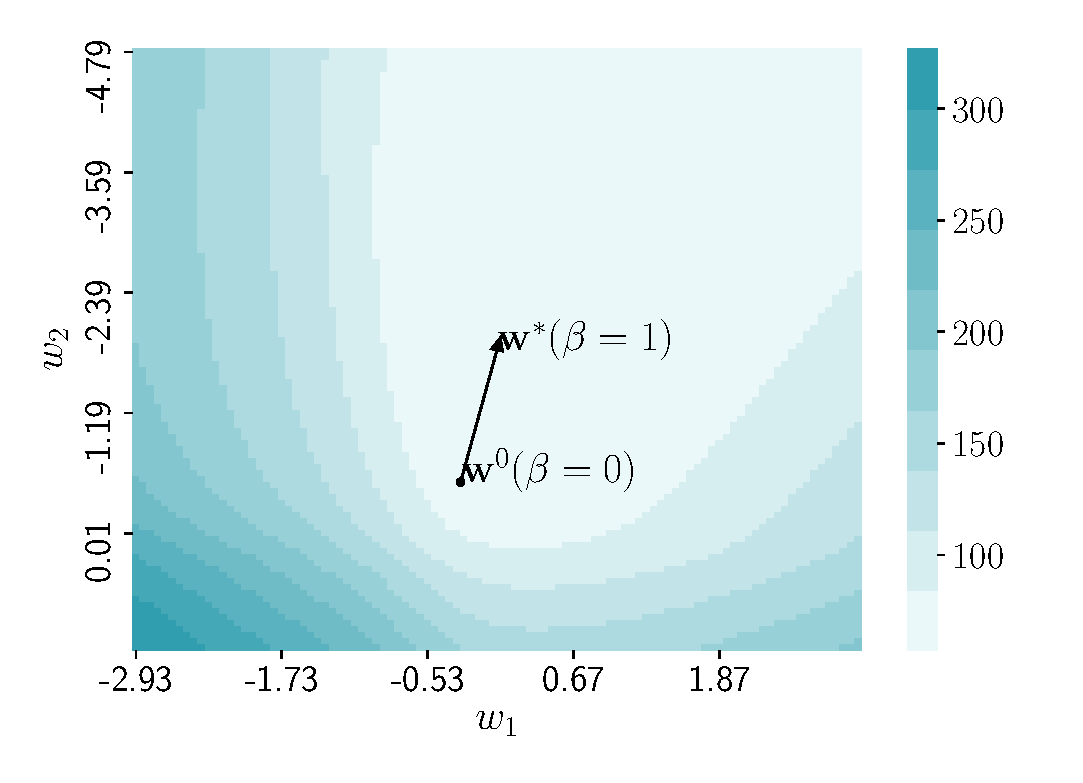
\includegraphics[width=\linewidth]{figs/ch3/neural_error}
		\caption{Поверхность функции ошибки для нейронной сети}
		\label{ch3:fig:neural_error}
	\end{minipage}%
	\begin{minipage}{.5\textwidth}
		\centering
		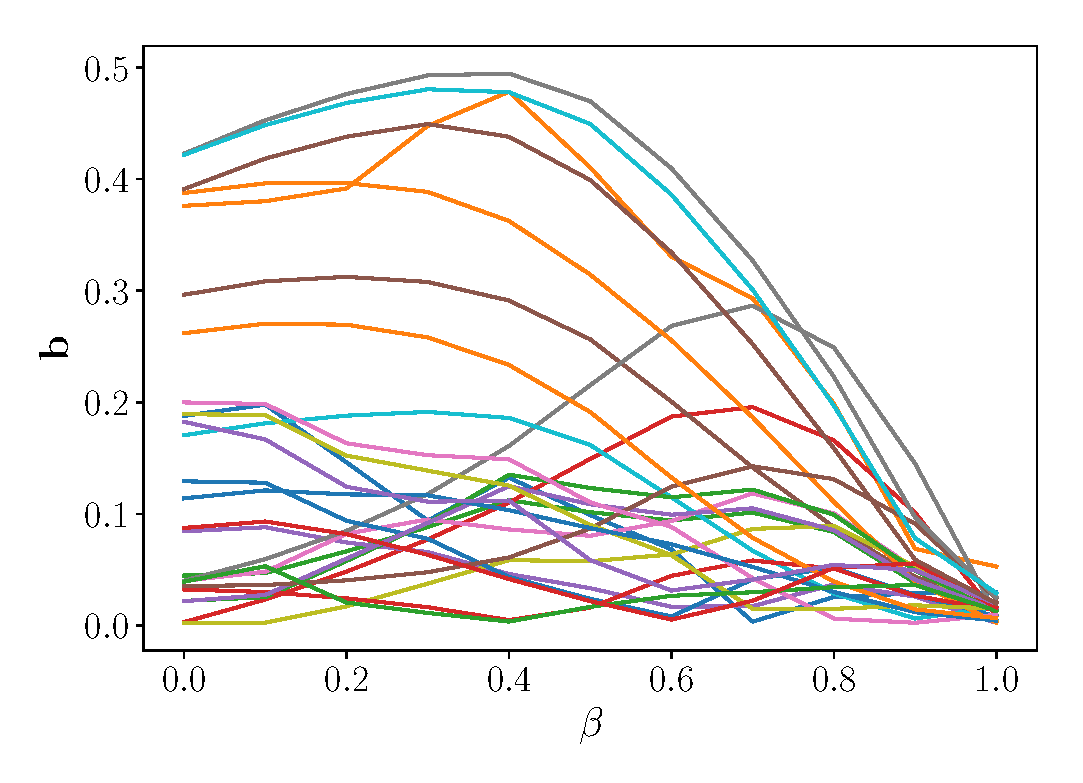
\includegraphics[width=\linewidth]{figs/ch3/neural_b_wrt_beta}
		\caption{Релевантность параметров первого слоя для модели нейронной сети}
		\label{ch3:fig:neural_b_wrt_beta}
	\end{minipage}
\end{figure}

На Рис.~\ref{ch3:fig:irls_qpfs_2d} показан процесс оптимизации для предложенного алгоритма в случае логистической регрессии с двумя параметрами модели. 
Даже для двумерной задачи решение метода Ньютона нестабильно и число обусловленности матрицы Гессиана~$\bH$ может быть чрезвычайно большим. 
На каждом шаге алгоритма процедура QPFS выбирает параметры для оптимизации. 
В данном примере предложенный алгоритм выбирает и обновляет только один параметр на каждой итерации на первых шагах. 
Это делает алгоритм более устойчивым.

\begin{figure}[!ht]
	\centering
	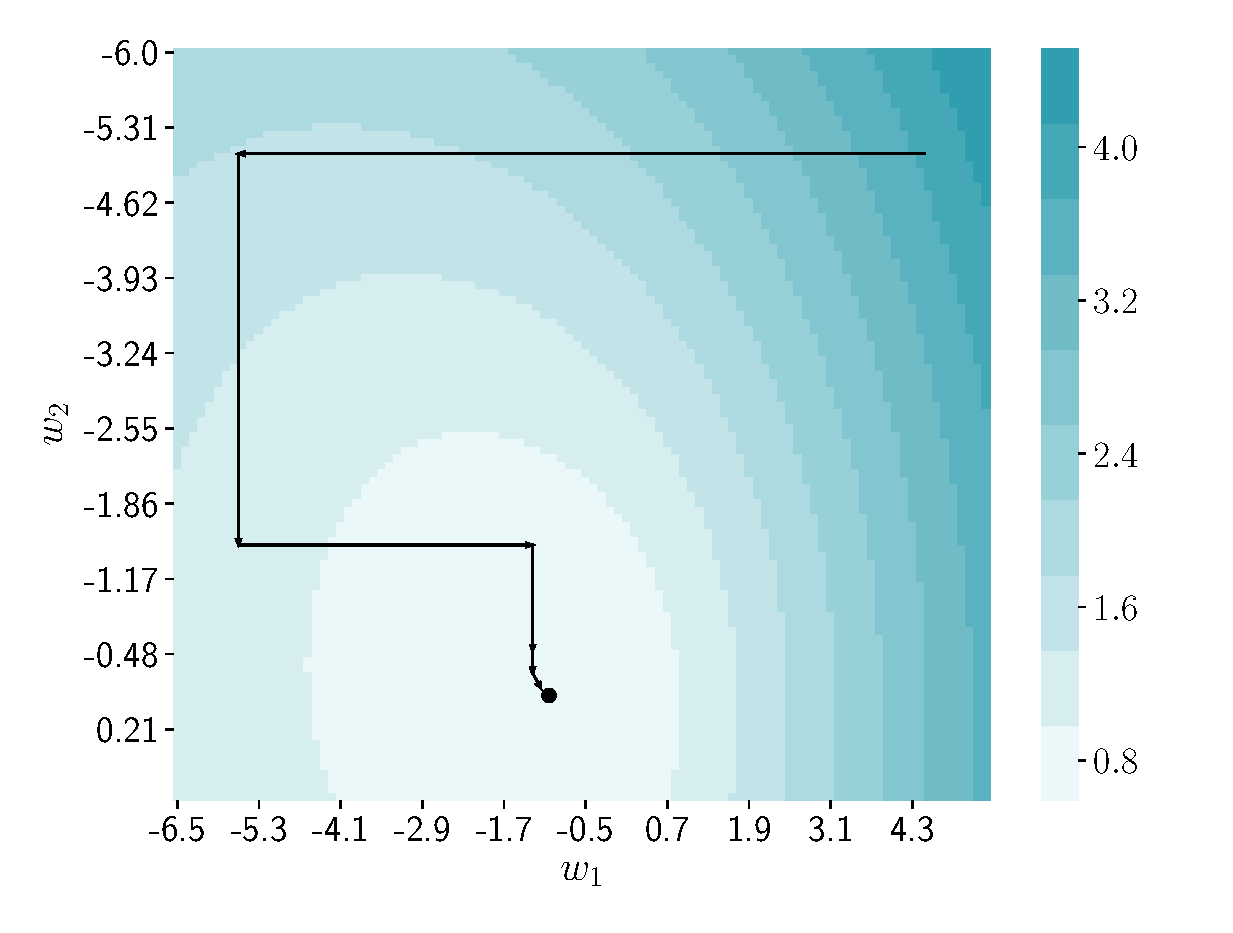
\includegraphics[width=0.6\linewidth]{figs/ch3/irls_qpfs_2d}	 
	\caption{Оптимизационный процесс предложенного алгоритма QPFS+Ньютон для модели логистической регрессии}
	\label{ch3:fig:irls_qpfs_2d}
\end{figure}

На Рис.~\ref{ch3:fig:active_params_wrt_iters} показаны наборы активных параметров на итерациях для набора данных Boston Housing и нейронной сети с двумя скрытыми нейронами. 
Темные ячейки соответствуют активным параметрам, которые мы оптимизируем.
 
\begin{figure}[!ht]
	\centering
	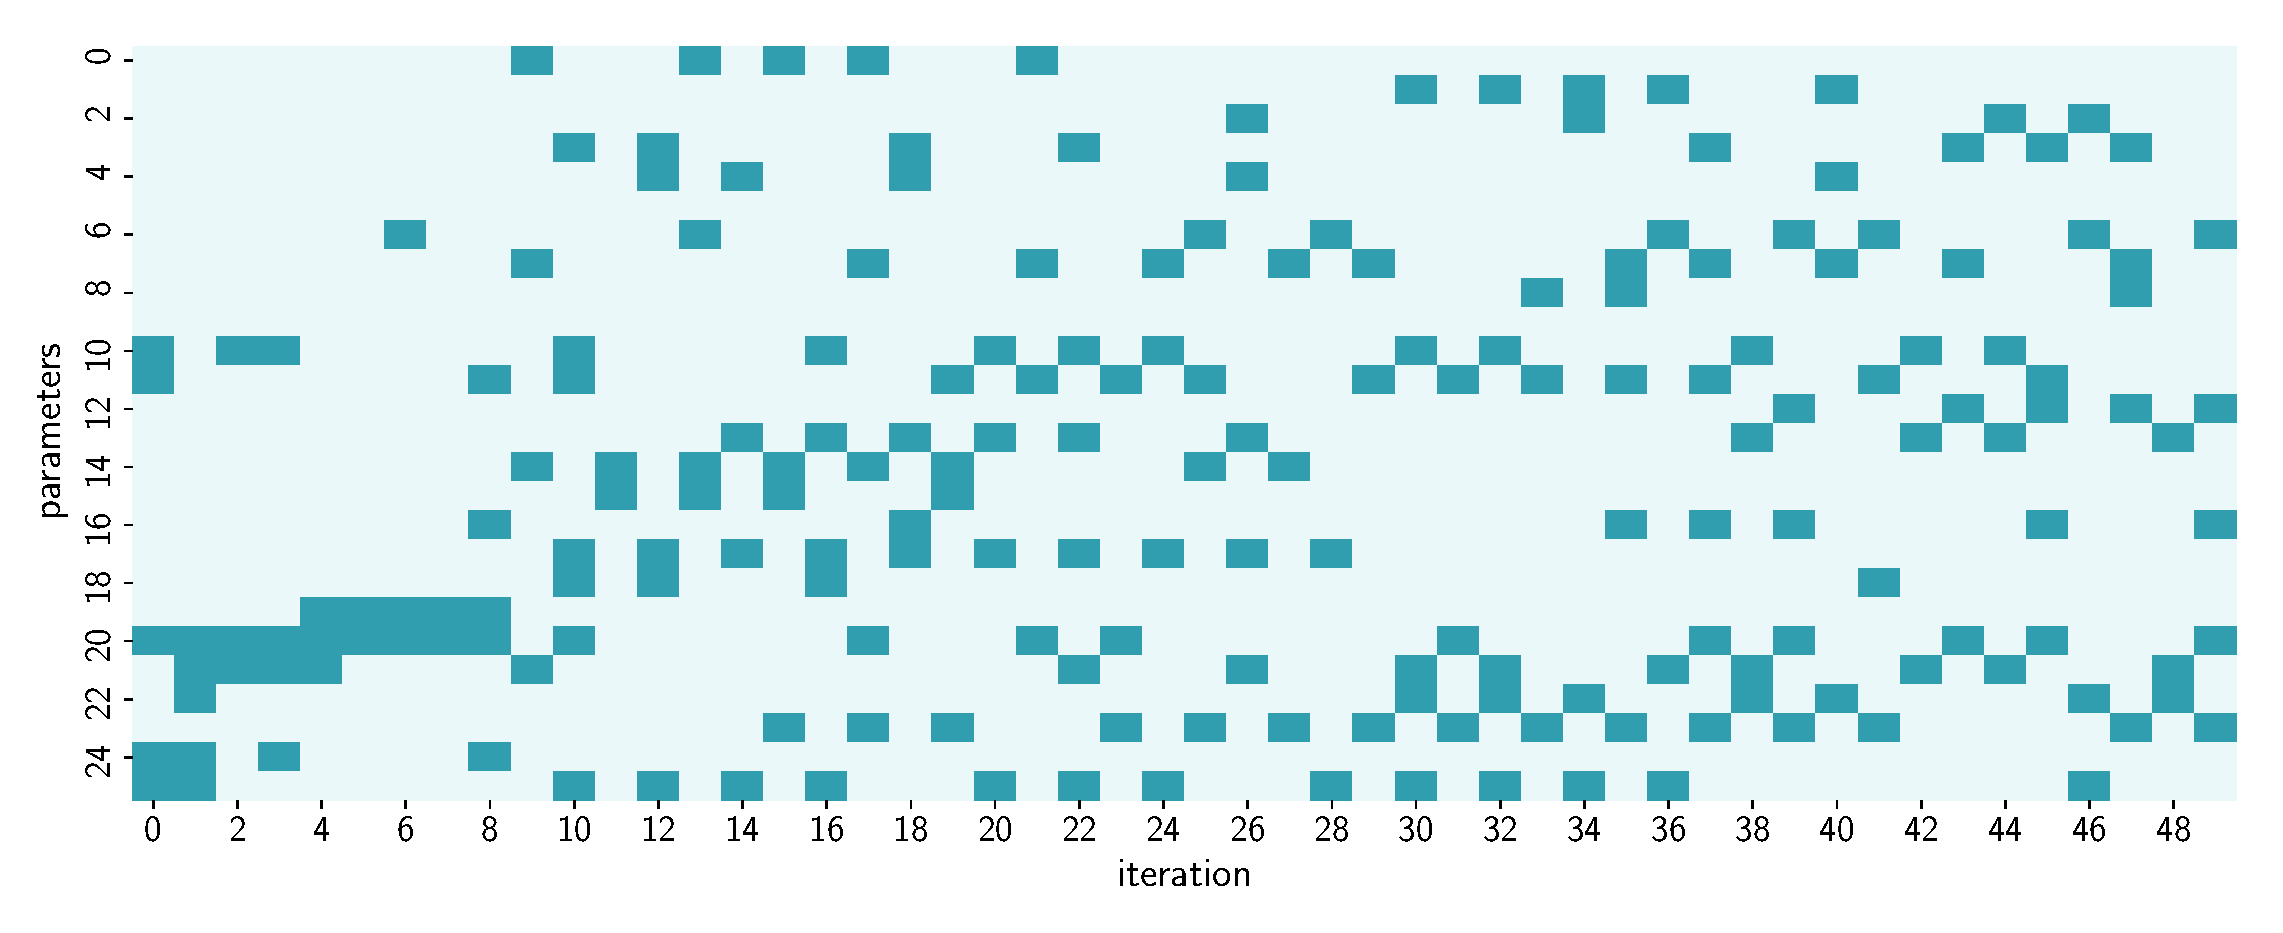
\includegraphics[width=\linewidth]{figs/ch3/active_params_wrt_iters}	
	\caption{Множество активных параметров на протяжении оптимизационного процесса}
	\label{ch3:fig:active_params_wrt_iters}
\end{figure}

В рассмотренных примерах число обусловленности~$\kappa(\bH)$ для метода Ньютона на некоторых итерациях было чрезвычайно большим. 
Выбор активных параметров позволил значительно сократить число обусловленности. 

Мы сравнили предложенный алгоритм с существующими методами, а именно градиентным спуском~(GD), моментом Нестерова, Adam и оригинальным алгоритмом Ньютона. 
Проведены эксперименты для моделей нелинейной и логистической регрессий. 
Наборы данных были выбраны из репозитория UCI~\cite{uci2017}. 
Результаты показаны в таблицах~\ref{ch3:tbl:nonlin_reg_results} и \ref{ch3:tbl:log_reg_results}. 
Для каждого набора данных две строки содержат ошибки для тренировочной~(первая строка) и тестовой~(вторая строка) выборок. 
В таблице~\ref{ch3:tbl:nonlin_reg_results} приведена квадратичная ошибка, в таблице~\ref{ch3:tbl:log_reg_results}~-- кросс-энтропия.
Чтобы найти среднюю ошибку и ее стандартное отклонение использовалась процедура кросс валидации на 5 фолдов. 
Предложенный алгоритм показывает меньшую ошибку на трех из четырех наборов данных для нелинейной регрессии и среди двух из трех наборов данных для логистической регрессии.

\begin{table}[!ht]
\footnotesize
	\caption{Средняя квадратичная ошибка на тренировочной и тестовой выборках для модели нелинейной регрессии}
	\label{ch3:tbl:nonlin_reg_results}
	\centering
	\begin{tabular}{|l|c|c|c|c|c|c|}
		\hline
		Выборка & \begin{tabular}[c]{@{}c@{}}\ $m$ \\ \ $n$ \end{tabular} 
		& GD 
		& Нестеров 
		& ADAM 
		& Ньютон 
		&
		\begin{tabular}[c]{@{}c@{}}QPFS+Ньютон\\ \end{tabular} \\ 
		\hline
		Boston House
		& 506
		& $27.2\pm4.6$
		& $46.0\pm11.0$
		& $35.4\pm2.5$           
		& $22.1\pm15.2$            
		& $20.9\pm10.4$   \\  
		Prices
		&\multicolumn{1}{c|}{13}
		& \multicolumn{1}{c|}{$32.4\pm5.6$}
		& \multicolumn{1}{c|}{$53.3\pm11.5$}
		& \multicolumn{1}{c|}{$37.8\pm7.0$}
		& \multicolumn{1}{c|}{$28.9\pm13.6$}
		& \multicolumn{1}{c|}{$\mathbf{24.5\pm9.4}$}\\ 
		\hline
		Communities
		& 1994
		& $48.0\pm6.4$
		& $31.4\pm2.8$
		& $23.3\pm3.7$        
		& $18.3\pm3.4$          
		&  $26.7\pm3.1$  \\ 
		and Crime
		&\multicolumn{1}{c|}{99}
		& \multicolumn{1}{c|}{$47,5\pm6.5$}
		& \multicolumn{1}{c|}{$32.9\pm4.3$}
		& \multicolumn{1}{c|}{$28,1\pm4.5$}
		& \multicolumn{1}{c|}{$28.8\pm3.6$}
		& \multicolumn{1}{c|}{$\mathbf{28.4\pm3.0}$} \\ 
		\hline
		Forest
		& 517
		& $18.9\pm0.4$
		& $1.83\pm0.4$
		& $1.81\pm0.6$             
		& $17.7\pm0.4$             
		& $17.9\pm0.4$   \\ 
		Fires
		&\multicolumn{1}{c|}{10}
		& \multicolumn{1}{c|}{$\mathbf{20.0\pm2.1}$}
		& \multicolumn{1}{c|}{ $20.2\pm2.2$}
		& \multicolumn{1}{c|}{ $\mathbf{20.0\pm2.0}$}
		& \multicolumn{1}{c|}{ $20.6\pm1.4$}
		& \multicolumn{1}{c|}{ $20.2\pm2.2$} \\ 
		\hline
		Residential
		& 372
		&  $51.6\pm17.7$
		&  $32.6\pm19.5$
		&  $30.0\pm24.8$            
		&  $35.5\pm24.7$            
		&   $30.3\pm10.7$ \\ 
		Building
		&\multicolumn{1}{c|}{103}
		& \multicolumn{1}{c|}{ $53.7\pm13.9$}
		& \multicolumn{1}{c|}{ $34.1\pm13.6$}
		& \multicolumn{1}{c|}{ $34.1\pm19.4$}
		& \multicolumn{1}{c|}{ $35.0\pm15.6$}
		& \multicolumn{1}{c|}{ $\mathbf{30.9\pm5.3}$} \\ 
		\hline
	\end{tabular}
\end{table}

\begin{table}[!ht]
\footnotesize
	\caption{Среднее значение кросс-энтропии на тренировочной и тестовой выборках для модели логистической регрессии}
	\label{ch3:tbl:log_reg_results}
	\centering
	\begin{tabular}{|l|c|c|c|c|c|c|}
		\hline
		Выборка & \begin{tabular}[c]{@{}c@{}}\ $m$ \\ \ $n$ \end{tabular} 
		& GD 
		& Нестеров 
		& ADAM 
		& Ньютон 
		&
		\begin{tabular}[c]{@{}c@{}}QPFS+Ньютон\\ \end{tabular} \\ 
		\hline
		Breast
		& 569
		& $0.6\pm0.1$
		& $0.4\pm0.1$
		& $0.8\pm0.2$           
		& $0.3\pm0.1$            
		& $0.2\pm0.1$   \\  
		Cancer
		&\multicolumn{1}{c|}{30}
		& \multicolumn{1}{c|}{$\mathbf{0.9\pm0.2}$}
		& \multicolumn{1}{c|}{$1.0\pm0.7$}
		& \multicolumn{1}{c|}{$1.2\pm0.2$}
		& \multicolumn{1}{c|}{$1.0\pm0.2$}
		& \multicolumn{1}{c|}{$1.1\pm0.3$}\\ 
		\hline
		Cardiotocography
		& 2126
		& $11.5\pm4.7$
		& $11.5\pm4.7$
		& $8.8\pm4.4$        
		& $11.5\pm5.7$          
		&  $7.7\pm4.2$  \\
		
		&\multicolumn{1}{c|}{21}
		& \multicolumn{1}{c|}{$11.6\pm5.8$}
		& \multicolumn{1}{c|}{$11.5\pm5.7$}
		& \multicolumn{1}{c|}{$9.0\pm2.6$}
		& \multicolumn{1}{c|}{$11.5\pm4.7$}
		& \multicolumn{1}{c|}{$\mathbf{7.7\pm4.7}$} \\ 
		\hline
		Climate Model
		& 540
		& $1.2\pm0.1$
		& $1.0\pm0.2$
		& $1.5\pm0.2$             
		& $1.0\pm0.5$             
		& $0.8\pm0.3$   \\ 
		Simulation Crashes
		&\multicolumn{1}{c|}{18}
		& \multicolumn{1}{c|}{$1.4\pm2.0$}
		& \multicolumn{1}{c|}{ $1.3\pm0.7$}
		& \multicolumn{1}{c|}{ $1.8\pm0.3$}
		& \multicolumn{1}{c|}{ $1.2\pm0.5$}
		& \multicolumn{1}{c|}{ $\mathbf{1.1\pm0.4}$} \\ 
		\hline
	\end{tabular}
\end{table}

